\documentclass[10pt,conference,compsocconf]{IEEEtran}

\usepackage[hidelinks]{hyperref}
\usepackage{graphicx}	% For figure environment
\usepackage{amsmath} % for mathematical symbols and environments
\usepackage{amssymb} % for mathematical symbols
\usepackage{amsfonts} % for mathematical fonts
\usepackage{bbm} % for blackboard bold symbols
\usepackage{setspace} % for blackboard bold symbols

\begin{document}
\title{Stochastic Gradient Quantization : \\ Saving Bandwidth in Distributed Learning}

\author{
  Salim Zrouga, Dominik Frey, Emilien Guandalino\\
  \textit{École Polytechnique Fédérale de Lausanne, Switzerland}
}

\maketitle

\begin{abstract}

	With the ever-increasing size of machine learning models, and with the development of scale-out architectures, distributed learning has become crucial to exploit the benefits of parallelism. Stochastic Gradient Descent (SGD) is naturally suited for this task as it can leverage the distribution of data. However, the necessary exchange of gradients among workers leads to bandwidth limitations becoming a new performance bottleneck. Quantized SGD (QSGD) addresses this issue through quantization of gradients before their exchange. This report aims to analyze the practical effects on convergence of such lossy compression schemes.
\end{abstract}

\section{Introduction}

Distributed learning provides scalable and elastic compute power for model training. 
However as the number of nodes increases, communication can saturate bandwidth limitations and cause large overheads.
QSGD \cite{quant} proposes gradient quantization to trade-off lower bandwidth usage for higher variance during training, and shows that models will still converge to local optima. The paper gives two algorithmic ideas : a stochastic gradient quantization scheme and an efficient encoding of quantized gradients. In this report, we will only be concerned about the first idea and we will analyze the effects of gradient quantization on convergence rates in practice.

We will be presenting the results of training 3 popular models in a distributed settings with different quantization rates. Remarkably, we found that in our applications we can reduce bandwidth usage by at least 3.6x without any percieved downsides, and up to 6.4x with minor increase on convergence time. In terms of network accuracy, quantized training converges towards each model's top accuracy and often generalizes better on the test set.

\section{Technical Background}

Quantization is a signal processing technique in which continuous values are mapped to a discrete subset of the value range. This enables values to be encoded in a space efficient manner while preserving most of the original information. This quantization can be deterministic, and map to the closest discrete value, or stochastic and map to discrete values with probability proportional to their distance, see Fig. \ref{fig:quant}. 

\begin{figure}[b]
  \centering
  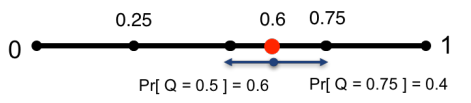
\includegraphics[scale=0.45]{quant}
  \caption{Stochastic Quantization}
  \vspace{-3mm}
  \label{fig:quant}
\end{figure}

QSGD defines a stochastic quantization scheme for $s$ quantization levels of $v \in \mathbb{R}^{n}$, $v \neq 0$ :
\[Q_s(v_i) = {\lVert v \rVert}_2 \cdot \text{{sgn}}(v_i) \cdot \xi_i(v, s)\]
where $\xi_i(v, s)$'s are independent random variables defined as follows : Let $0 \leq k < s$ be an integer such that $\frac{{\lvert v_i \rvert}}{{\lVert v \rVert}_2} \in [\frac{k}{s}, \frac{k + 1}{s}]$. That is, $[\frac{k}{s}, \frac{k + 1}{s}]$ is the quantization interval corresponding to $\frac{{\lvert v_i \rvert}}{{\lVert v \rVert}_2}$. Then,
\[\xi_i(v, s) = \begin{cases}
\frac{k}{s} & \text{{with probability }} 1 - p\left(\frac{{\lvert v_i \rvert}}{{\lVert v \rVert}_2}, s\right), \\
\frac{k + 1}{s} & \text{{otherwise}}.
\end{cases}\]
With $p(a, s) = as - k$ for $a \in [0, 1]$. If $v = 0$, then we define $Q(v, s) = 0$. 

Intuitively, $k$ is the 0-based index to which the value will be mapped in the interval, for example 2 or 3 in Fig. \ref{fig:quant}. The $\xi_i(v, s)$'s are then the corresponding values at that index, 0.5 or 0.75 in our example.

Once this quantization is done, we exchange gradients using the simple encoding given bellow :

\vspace{-0.6em}
\singlespacing
\noindent \emph{Encoding} : For a $n$ dimension vector with $q = log_2(s)$ quantization bits, send 32 bits for the norm, $n$ bits for the sign vector, and the $n$ quantization indices $k$ of $q$ bits each, from which $\xi_i(v, s)$ can be recovered.
\vspace{-0.6em}
\singlespacing
We therefore estimate the bandwidth usage in number of bits sent as such :

\begin{center}
 \# bits = $32 + n + q * n$
\end{center}

QSGD actually proposes a more clever encoding, but this one is simple enough and sufficient for our analysis.

\section{Experiments}

\subsection{Model Definition}

\subsubsection{Dataset}

We will conduct our experiments on an image classification task on the CIFAR-10 dataset. It contains 60,000 colored 32x32 pixel images, with 10 differents classes. We will be using 50,000 samples for training, with a 0.1 validation split (5,000 samples), and the remaining 10,000 samples are used for testing.

\subsubsection{Models}

We train 3 popular models for image classification : AlexNet, ResNet18 and ResNet50. 

\noindent \textbf{AlexNet:} AlexNet is a deep convolutional neural network which achieved state of the art performance on the ImageNet challenge. Our implementation \cite{alexnet} has a total of 58 million parameters.

\noindent \textbf{ResNet:}
The ResNet architecture is built upon VGG networks. In order to train deeper networks and to circumvent the problem of vanishing gradients, the ResNet architecture in general includes skip connections between convolutional layers. These skip connections add the output from the previous layer to the layer ahead via an identity mapping, i.e. it does not apply any modification the the output from the previous layer \cite{resnet}:
\begin{align*}
    y = \mathcal{F}(x) + x
\end{align*}
However, sometimes these outputs do not have the same dimensions, as we perform the convolution operation. To fix this, the identity mapping is multiplied by a linear projection $W$ in order to match the size of the different outputs \cite{shorten}:
\begin{align*}
    y = \mathcal{F}(x, \{W_i\}) + W_d \times x
\end{align*}

All ResNet variants have 5 different kinds of convolutional layers. The ResNet architectures then differ in the number of convolutional layers for each of these five kinds, which always stay in the same proportions.


\subsubsection{Optimization}

As mentioned earlier, SGD is well suited for distributed learning tasks as it can take advantage of the data parallelism. We therefore split our data accross nodes, perform computation per node, and then average out the gradients. Quantization of the gradients is added at each node level before global averaging. We will be presenting results for up to 2, 4 and 8 bit quantization.

\subsubsection{Error correction}

The compression of gradients introduces an approximation error called quantization error. We can mitigate this information loss during training with a process we will call error correction. Upon each iteration, we remember the quantization error and add it to the gradient on the next iteration before quantization. This preserves more information in expectation accross iterations.

\subsubsection{Evaluation Method}

For each model, we first train a baseline model and compare based on the following three metrics :

\begin{itemize}
	\item[--] \textit{Accuracy :} Do we reach the same top test accuracy as the baseline model ?
	\item[--] \textit{Convergence Time :} How many epochs do we train until we reach top baseline accuracy ?
	\item[--] \textit{Bandwidth saving estimates :} What ratio of bytes are we saving per iteration per node ? This is based on the basic encoding we defined in the technical background section and could be improved using more clever encondings.
\end{itemize}

\subsection{Simulating Distributed Training}

Distributed training is difficult to implement properly and requires to deal with multiple GPUs, message passing protocols, gradient encodings, and other tricky problems which are outside the scope of this project. We decided to simulate distributed training instead, using a single GPU which sequentially computes forward and backward passes, quantizes gradients, and averages them out on a single model. 

A good point is that we are still able to see the negative effects of quantization on convergence rates, in terms of number of iterations. However, a major drawback is that since we are not actually broadcasting the gradients, we cannot truly measure improvements on communication costs. When using quantization for bandwidth reduction we essentially trade-off higher computation time for lower communication time. By balancing out this ratio, we decrease total training time, not in terms of iterations but in real time. This improvement cannot be measured quantitatively in our situation, only roughly estimated by looking at the number of bits saved per node.


\subsection{Results}

All the following experiments simulated a distributed settings with $n = 2$ nodes. We would expect similar results when running 4 or 8 nodes in terms of accuracy and convergence rate, although the real time speedup would be much greater. We first run a baseline experiment with no quantization, i.e. 32 bits and compare different quantization levels based on the previously mentioned criteria : Test Accuracy, Epochs to Convergence and Bandwidth Saving.

\textbf{AlexNet:} We used stochastic quantization, error correction, batch size per node $B = 64$, step size $\gamma = 0.005$, weight decay $w = 0.005$, and momemtum $m = 0.9$. 

\begin{table}[htbp]
  \centering
  \begin{tabular}[c]{|c||c|c|c|}
    \hline
	  Quantization&Accuracy&Epochs&Bandwidth\\
    \hline
	  32 bits&83.25\% &16&1x\\
	  8 bits&84.2\%&18&3.6x\\
	  4 bits&85.19\%&22&6.4x\\
	  2 bits&84.3\%&28&10.7x\\
    \hline
  \end{tabular}
	\vspace{0.7em}
	\caption{Training Results for AlexNet}
\end{table}

\vspace{-1.5em}
\noindent It is hard to estimate exactly when a model has converged to top test accuracy during training. We therefore saved the 3 models which performed the best on validation set and reported the greatest test accuracy out of the 3. Although some variance is always to be expected between experiments, we can see that there is a clear trend of increasing convergence time for coarser quantization levels. Between 32 bits and 2 bits quantization, the accuracy is better by 1.05\%, the convergence time is about 1.75x longer, but the amount of saved bandwidth is 10.7x compared to baseline.
\vspace{0.3em}


\textbf{ResNet50:} As this model is quite big, we set the number of epochs to 20 in order to limit the running time. As for the parameters, we used stochastic quantization, error correction, batch size per node of $B = 128$, weight decay $w = 0.001$, step size $\gamma = 0.01$ and momentum $m = 0.9$.
\begin{table}[htbp]
  \centering
  \begin{tabular}[c]{|c||c|c|c|}
    \hline
          Quantization&Accuracy&Epochs&Bandwidth\\
    \hline
          32 bits&82.22\% &20&1x\\
          8 bits&82.78\%&16&3.6x\\
          4 bits&82.48\%&18&6.4x\\
          2 bits&81.56\%&20&10.7x\\
    \hline
  \end{tabular}
        \vspace{0.7em}
        \caption{Training Results for ResNet50}
\end{table}

\vspace{-1.5em}
We can observe an increasing accuracy for the number of quantization bits, where quantization with 8 bits converged the fastest to its top accuracy value.
As for bandwidth savings, they are a constant ratio which only depends on the number of bits of quantization. In terms of actual space saved, models with larger number of parameters will benefit more from quantization on each iteration.
\vspace{0.3em}

\textbf{ResNet18:} For this model, we used stochastic quantization, error correction, batch size per node of $B = 128$, weight decay $w = 0.001$, step size $\gamma = 0.01$ and momentum $m = 0.9$.

\begin{table}[htbp]
  \centering
  \begin{tabular}[c]{|c||c|c|c|}
    \hline
	  Quantization&Accuracy&Epochs&Bandwidth\\
    \hline
	  32 bits&86.98\% &30&1x\\
	  8 bits&87.06\%&27&3.6x\\
	  4 bits&87.15\%&30&6.4x\\
	  2 bits&86.82\%&32&10.7x\\
    \hline
  \end{tabular}
	\vspace{0.7em}
	\caption{Training Results for ResNet18}
\end{table}
\vspace{-1.5em}


Here, we used early stopping to determine when the model had converged. If the performance on the validation set has not improved after a certain number of epochs, called "patience", the training ends and we return the best performing model.
\vspace{0.3em}


\subsection{Discussion}


Overall, the results seem to confirm what is presented in the QSGD paper, that is, as the quantization level gets smaller, models take longer to converge to their top accuracy. On the good side, models with quantized training are consistently better in test accuracy than the baseline models, which we can assume to be due to less overfitting from lower precision gradients. This obviously has a limit, as a too aggressive quantization will eventually degrade top accuracy.

\textit{Communication costs:} Concerning bandwidth saving estimates, once again it is hard to say how much the real time speedup would be from this. However, if bandwidth limitation is saturated, waiting times grow exponentially which may lead to massive communication overheads. Preventing this from happening on each iteration is most likely worth the extra number of convergence epochs. 

\textit{Computation Costs:} When comparing with the baseline run, quantization added a massive overhead in computation time (at least 3x), especially when running stochastic quantization instead of deterministic one. We tried training with determinstic quantization, which yielded smaller running times, but this affected top accuracy. For AlexNet, when training for 2 bits, the model never scored better than 73\% of test score, even with a large number of epochs. We believe that this increase of computation is due to the expensive nature of generating a random number for each quantized value, but this overhead is necessary to reach top accuracy. In truly distributed applications, those computation costs would be parallelized, but would still represent a substantial increase.


\begin{center}
\textit{Perfectly balanced, as all things should be..}
\end{center}

As with most engineering concepts, we are trading-off between two magnitudes to achieve optimal performance. In our situation, we are willing to increase the number and the cost of iterations in order to reduce gradient exchange times. Quantization enables this fine-tuning between computation costs and communication costs to happen smoothly. We can therefore optimize appropriately each model and achieve real time speedup.


\section{Summary}

We have presented 3 practical implementations of gradient quantization on deep convolutional neural networks, and have observed the effects on convergence. At a high level, quantization increases the number of iterations to convergence in order to reduce communication times. It is quite remarkable that with 8 bits quantization, we can achieve similar performance to baseline for almost no increase in convergence time, and reduce bandwidth usage by at least 3.6x. We also provide all the necessary code to reproduce our experiments.

\section*{Acknowledgements}

We would like to thank the authors of the QSGD paper for their amazing work and interesting paper. We would also like to thank the developers who publicly made available their implementation and training of the networks. This enabled us to spend most of our time on the interesting parts of the project. Last but not least, we would like to thank our corrector for taking the time to read through our work.

\singlespacing
\singlespacing
%\newpage
\bibliographystyle{IEEEtran}
\bibliography{references}

\end{document}
